%TO-DO
%
% add figures, both for normal cases and for specific metrics
% [ IV in CBC vs CFB ]
% review pls!

\documentclass[11 pt]{article}
\usepackage{graphicx}
\title{
	Study and Implementation of AES-128 in Python3 \\
	\large Homework 2 - CNS Sapienza}

\author{Lauterio Davide 1934615}
\date{30/10/2020}

\begin{document}

\maketitle


\section{Objective}
The point of this homework was to:
\begin{itemize}
\item Implement AES-128
\item Extend that implementation adding at least 3 operation modes [ECB, CBC, CFB, OFB, CTR]
\item Provide experimental comparison between our implementation and a well-known one.
\end{itemize}


\section{What is AES}

Advanced Encryption Standard (AES) or Rijndael in its first implementation is a symmetric block cipher with 128 bits blocks.
Rijndael was originally written for a challenge to create a new block cipher announced by NIST in January 1997.
As now, it is one of the most used symmetric cipher, even suggested from US federal standard.

\subsection{How AES Works}
Speaking about a single 16 Bytes block and a 16 Bytes key.
At the start the input of the algorithm is encoded in a 4x4 matrix called State and the key is "expanded" in a one dimensional array of four-byte words derived using the Key Expansion routine described in Section 5.2 of "FIPS 197".
The key vector and the state matrix will be processed by 4 layers for n times, where n is a number of rounds given depending the length of the key.
The layers are: 
\paragraph{Byte Substitution/Confusion Layer}
In this layer is used an "S-Box" to produce a non linear byte substitution, operated independently on each byte/cell of the state matrix.
An S-Box is constructed starting from a finite  field  $GF(2^8)$, in which the first element {00} is mapped to itself. For this implementation the S-Box is taken precomputed on Matlab.
Every part of this algorithm is linear except this layer which is reversible because bijective, i.e., there exists a mapping of every input to every output.
\begin{center}
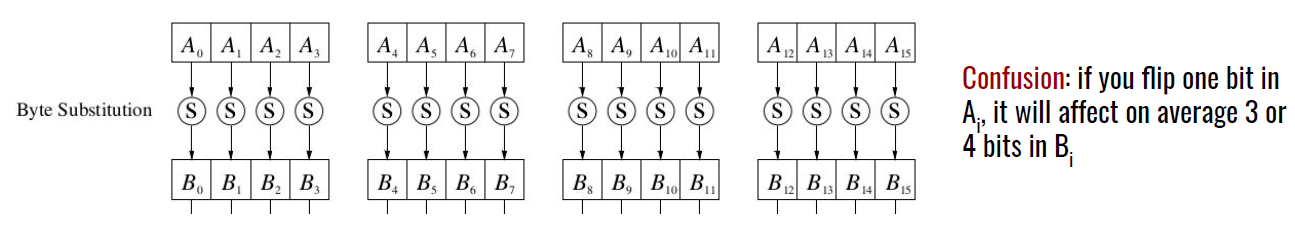
\includegraphics[width=1\textwidth]{ByteSub_Slides.png}
\end{center}
\paragraph{Diffusion Layer}
This layer is divided in two parts and it serve to diffuse the "confusion" added in the previous layes, as it may be obvious by the name.
\begin{center}
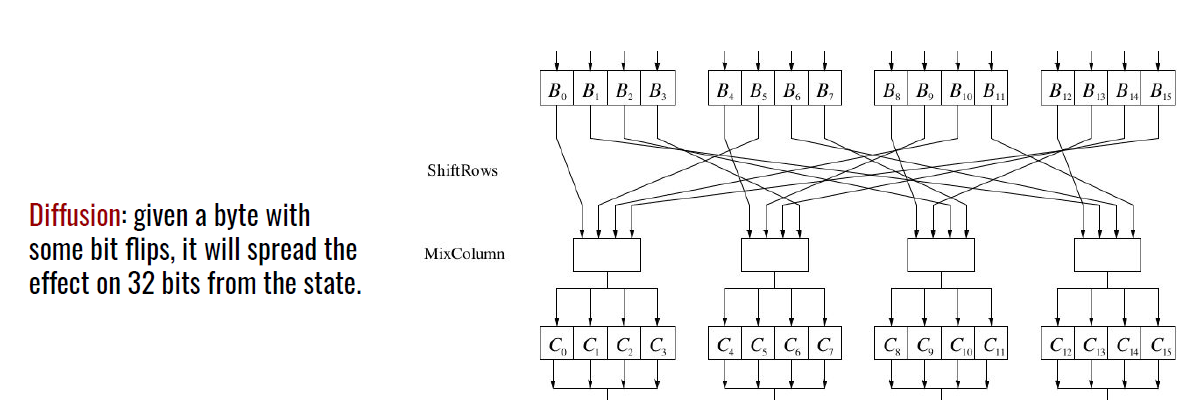
\includegraphics[width=0.75\textwidth]{Diffusion_Slides.png}
\end{center}
\subparagraph{Shift Rows Layer}
This layer is called every round after the byte subtitution. In this transformation the bytes in the last three rows of the State are cyclically shifted over different numbers of bytes (offsets). The first row, $r = 0$, is not shifted.
\begin{center}
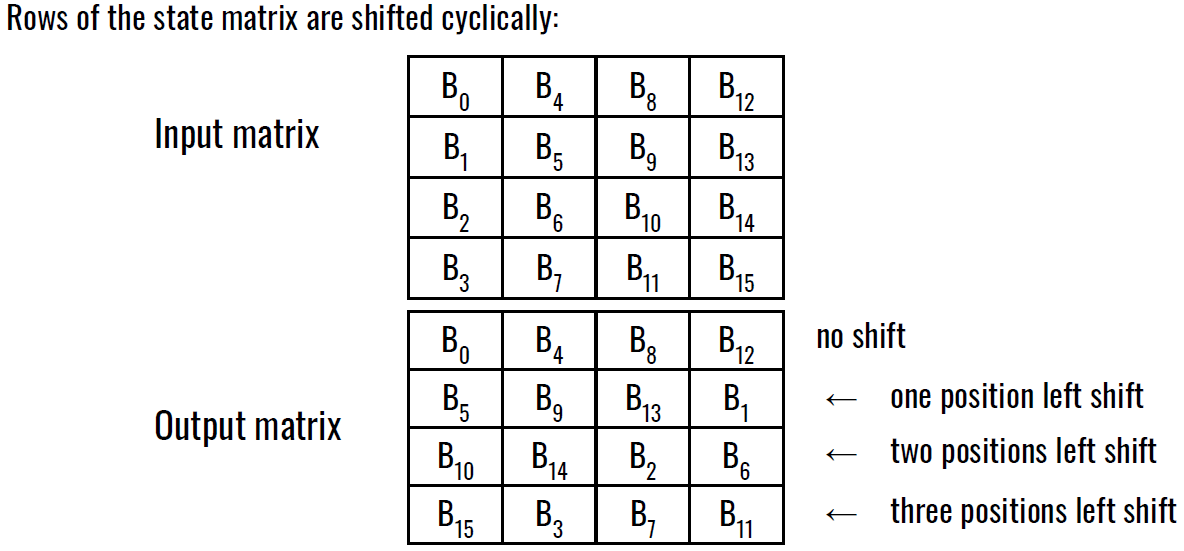
\includegraphics[width=0.75\textwidth]{ShiftRows_Slides.png}
\end{center}
\subparagraph{Mix Column Layer}
This layer compose the second half of the Diffusion Layer. Executed every round after the shift rows operation except for the last round in which it is skipped. 
Each 4 Byte column of the state is considered as a vector and multiplied(XOR) by a fixed matrix.
All arithmetic is done in the $GF(2)$.
\begin{center}
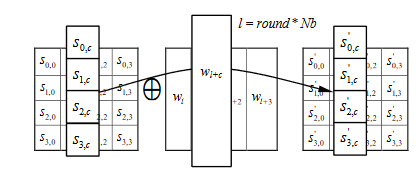
\includegraphics[width=0.75\textwidth]{MixColumns_Slides.png}
\end{center}
\paragraph{Key Addition/Whitening Layer}
In the key whitening transformation, a Round Key is added to the State by a simple bitwise XOR operation.  Each Round Key consists of Nb words from the key schedule, obtainedby the key expansion.
\subparagraph{Key Expansion}
The AES algorithm takes the Cipher Key, K, and performs a Key Expansion routine to generate a key schedule. The Key Expansion generates a total of $Nb$ ($Nr$ + 1) words: the algorithm requires an  initial  set  of  Nb  words,  and  each  of  the  $Nr$  rounds  requires  $Nb$  words  of  key  data.    The  resulting key schedule consists of a linear array of 4-byte words, denoted [$w_i$], with i in the range $0 <= i < Nb(Nr + 1)$.
\begin{center}
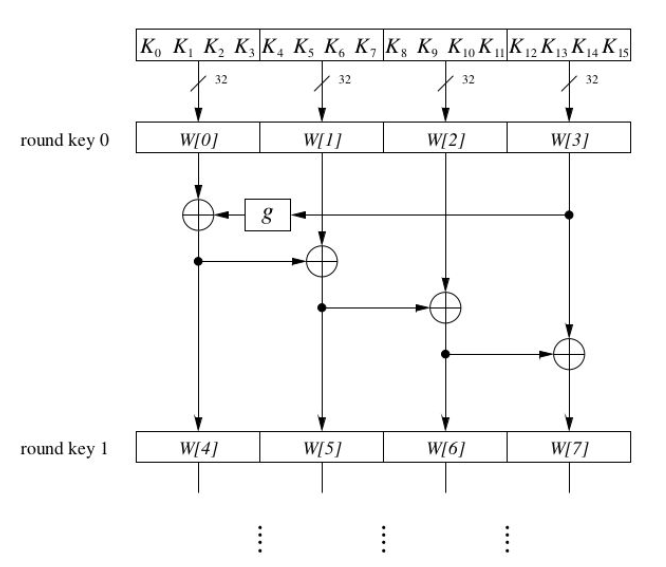
\includegraphics[width=0.5\textwidth]{KeyExp_Slides.png}
\end{center}


\section{Implementation and Conclusions}
To come across this homework I had to learn both, the teorical implementation of AES and the Python language.
This was, of course, a problem too big to be tackled as once, so I've started putting on paper sketches of the algorithm. The fact that it is itself divided in layer made it easier.
I've started researching other implementations, in the python language and not, to learn to recognise every block in every implementation i found.

The first layer implemented was diffusion layer, which is practically easier.
I've followed the instruction found on "The Rijndael Design" section 4, and this was basically 1 out of 3 done.

The substitution layer was also not a big deal by itself, but i wanted to compute the S Boxes, so not knowing SageMath I've tryed to get them out of matlab. I'll put the code on GitHub too after some polishing, then I've copy-pasted the matrix and the inverted one for the decryption.

The Key Addition method was the same as the byte substitution, but i was still missing the key extension part. I've ended up putting it in the AES class, so given the original key at the initialization of it the key will be expanded before starting encyption or decryption.

After all layers were complete, I've started coding the encryption and decryption of a single block and then made a method that accepted a long input, subdivided it in 16 Bytes blocks and encrypted block by block.
The input must still be multiple of 16 Bytes.

To test I went for the simplest thing that came in my mind, I made a simple random string generator.

Due to time limitation I could not implement any mode of operation and due to a bug relative to my machine I could not perform any comparison with a well known aes implementation, nonetheless I've managed to record the time my implementation takes to run for strings up to 1KB, 100 KB and 10 MB.

The long time taken to encrypt or decrypt must be caused by lateness given by the python which is a high level programming language. Probably with a language like C a shorter time is achievable.

Thank you for the attention.


% put after conclusion
\begin{thebibliography}{10}

	% bibitem for paper
	\bibitem{FIPS 197}
	 Federal Information Processing Standards Publication 179, published in 2001.	
	 \bibitem{Rijndael}
	 Joan Daemen, Vincent RijmenThe Design of RijndaelAES — The Advanced Encryption Standard, November 26, 2001
	
\end{thebibliography}

\end{document}
